\section{Planificación}

En este apartado haremos un breve recorrido por los recursos que utilizaremos a nivel software y hardware, ya que a nivel de recursos humanos es un proyecto de un solo estudiante (con la supervisión del tutor); mediante diagramas de Gantt veremos la planificación temporal del proyecto; hablaremos de la metodología de desarrollo escogida; y finalmente comentaremos la viabilidad del proyecto.

% ---------------------------------------------------------------------------- %

\subsection{Recursos}

\subsubsection{Hardware}
    
    \textbf{Equipo principal:} Equipo personal a medida
    \begin{itemize}
        \item \textbf{CPU:} Intel(R) Core(TM) i5-10500H 2.90GHz. 6 sockets con 2 núcleos/socket.
        \item \textbf{GPU:} Gigabyte GeForce RTX 3060 Ti EAGLE OC
        \item \textbf{RAM:} 16 GB
    \end{itemize}
    
    \textbf{Equipo secundario:} Lenovo IdeaPad 330
    \begin{itemize}
        \item \textbf{CPU:} Intel(R) Core(TM) i5-8300H 2.30GHz. 2 sockets con 4 núcleos/socket.
        \item \textbf{GPU:} NVIDIA GeForce RTX 1050
        \item \textbf{RAM:} 8 GB
    \end{itemize}

\subsubsection{Software}

\paragraph{Biblioteca gráfica: Three.js}

    Aunque habitualmente el uso de un lenguaje o una biblioteca específica no es más que un tema menor en el desarrollo de un proyecto, en este caso sí es un elemento a tener en cuenta, ya que al no usar un motor de juegos, se aporta un elemento de complejidad y un valor añadido al trabajo.\\
    
    Con ese fin se ha escogido la biblioteca de alto nivel para gráficos 3D en JavaScript, Three.js, que nos permite crear gráficos y animaciones 3D en un navegador web. Además es una biblioteca libre y disponible en GitHub \cite{githubThree}.\\
    
    El uso de esta herramienta frente a un motor de juegos clásico supondrá que todo lo relacionado con físicas, colisiones, controles, etc. quedará bajo nuestra responsabilidad, mientras que nos facilitará el tratamiento de gráficos y nos dará una mayor flexibilidad a la hora de desarrollar el proyecto.

\paragraph{Control de versiones: Git y GitHub}

    De cara a llevar un control de versiones y facilitar el seguimiento del desarrollo del proyecto, se ha decidido usar el software libre Git \cite{git}. El uso de esta herramienta facilitará seguir una metodología incremental a la hora del desarrollo, metodología de la que hablaremos más adelante.\\
    
    De manera complementaria a Git se utilizará la forja Github \cite{github} como plataforma de desarrollo colaborativa, ya que sirve para alojar proyectos que utilicen el control de versiones que nos ofrece Git. Aunque el proyecto a nivel de recursos humanos solo sea llevado por una persona, el uso de una plataforma colaborativa facilita el uso de dos equipos, el seguimiento del proyecto por parte del tutor y abre la posibilidad de compartir el proyecto e incluso desplegarlo con Github Pages \cite{githubPages}.

\subsection{Desarrollo}

\subsubsection{Diagrama de Gantt}

    Como parte de la planificación, se ha realizado un cronograma del proyecto mediante un diagrama de Gantt. El diagrama nos permitirá llevar un control del tiempo previsto para cada apartado del proyecto y realizar modificaciones en la planificación si es necesario. Inicialmente, se propone una planificación con una duración de 30 semanas.\\
    
    Entrando ya en la planificación propuesta, se ha divido la planificación del proyecto en los siguientes tres bloques principales:
    
    \begin{itemize}
        \item \textbf{Investigación:} refleja el tiempo previsto a emplear en el análisis del funcionamiento del juego como la propia investigación y autoaprendizaje sobre generación procedimental y cómo poder aplicarla a nuestro juego.
        \item \textbf{Desarrollo:} refleja el tiempo previsto a emplear en el desarrollo e implementación de la aplicación. Dividiremos la cronología en el juego en sí y los apartados relacionados con \acrshort{pcg}, previsiblemente siendo generación de escenarios, texturas e modificación de la dificultad y/o el comportamiento de la inteligencia artificial.
        \item \textbf{Documentación:} refleja el tiempo previsto a emplear la realización de la memoria del proyecto y de la inclusión de bibliografía en el mismo, por lo que en muchas ocasiones, se realizará en paralelo junto al apartado de investigación.
    \end{itemize}
    
    Mencionar que las semanas 8 y 9 se han dejado en blanco debido a que coinciden con el periodo de exámenes. También aclarar que aunque se incluye la semana 30, ha sido únicamente por una cuestión estética en la presentación del diagrama, ya esa semana forma parte de la entrega del proyecto.

    \begin{figure}[H]
    \begin{center}
        \begin{subfigure}[b]{0.95\textwidth}
            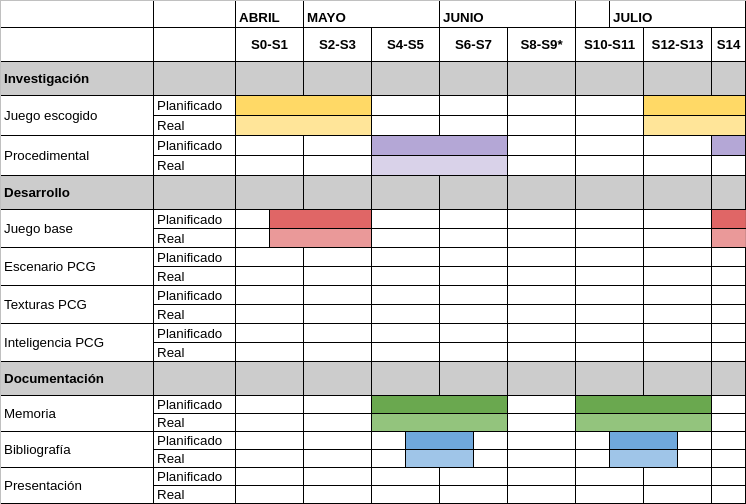
\includegraphics[width=\textwidth]{img/gantt-A.PNG}
            \caption{Planificación desde abril hasta julio.}
        \end{subfigure}
        \par\bigskip
        \begin{subfigure}[b]{0.95\textwidth}
            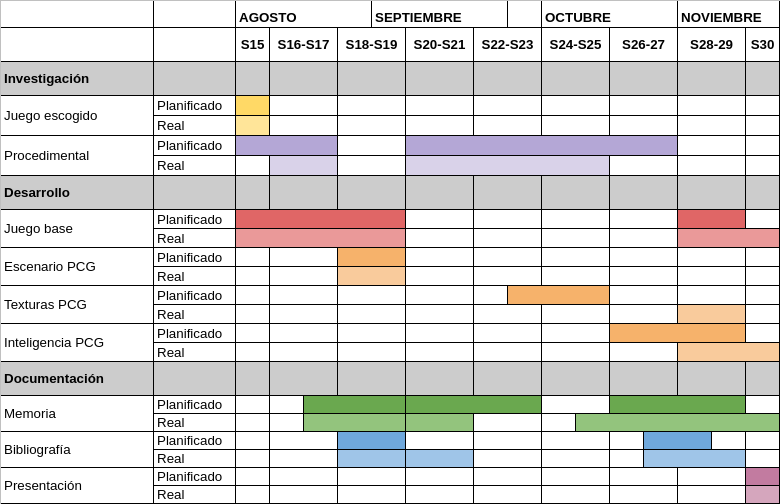
\includegraphics[width=\textwidth]{img/gantt-B.PNG}
            \caption{Planificación desde agosto hasta noviembre.}
        \end{subfigure}
        \caption{Diagrama de Gantt con el tiempo planificado y real para cada hito del proyecto.}
    \end{center}
\end{figure}
    
    
    \begin{table}[H]
        \centering
        \caption{Leyenda del diagrama de Gantt.}
        \begin{tabular}{|l|l|l|l|l|l|}
        \hline
        S0 & 19-25 abril       & S10 & 28 junio - 4 julio       & S20 & 6-12 septiembre         \\ \hline
        S1 & 26 abril - 2 mayo & S11 & 5-11 julio               & S21 & 13-19 septiembre        \\ \hline
        S2 & 3 - 9 mayo        & S12 & 12-18 julio              & S22 & 20-26 septiembre        \\ \hline
        S3 & 10 - 16 mayo      & S13 & 19-25 julio              & S23 & 27 septiembre-3 octubre \\ \hline
        S4 & 17-23 mayo        & S14 & 26 julio - 1 agosto      & S24 & 4-10 octubre            \\ \hline
        S5 & 24-30 mayo        & S15 & 2-8 agosto               & S25 & 11-17 octubre           \\ \hline
        S6 & 31 mayo - 6 junio & S16 & 9-15 agosto              & S26 & 18-24 octubre           \\ \hline
        S7 & 7-13 junio        & S17 & 16-22 agosto             & S27 & 25-31 octubre           \\ \hline
        S8 & 14-20 junio       & S18 & 23-29 agosto             & S28 & 1-7 noviembre           \\ \hline
        S9 & 21-27 junio       & S19 & 30 agosto - 5 septiembre & S29 & 8-14 noviembre          \\ \hline
        \end{tabular}
    \end{table}

\subsubsection{Metodología}

    De cara al modelo de trabajo, siendo un proyecto desarrollado por una sola persona, se plantea llevar una metodología incremental en la que se irán desarrollando, implementando y testeando las distintas funcionalidades que deba tener el juego escogido.\\
    
    Para ello y tal como puede ver en los diagramas de Gantt, se propone dividir el desarrollo en dos hitos con un peso similar, el juego base y la generación procedimental de contenidos, dividiéndose cada uno de ellos en distintas funcionalidades.\\
    
    Esta metodología nos permitirá ir desarrollando el proyecto en paralelo a la investigación sobre la \acrshort{pcg}, obteniendo a lo largo del mismo versiones funcionales del juego con las que realizar pruebas y mejoras durante todo el desarrollo.

\subsection{Viabilidad}

    A la vista de los recursos disponibles, siendo más que suficientes tanto en el apartado hardware como software; contando con un plazo de tiempo bien planificado y una planificación que permite modificaciones en caso de ser necesario; y siguiendo una metodología sencilla pero eficaz que facilita un desarrollo constante del proyecto a la vez que nos permite introducir cambios con facilidad en la aplicación; podemos concluir que el proyecto es viable en la forma y plazos planteados.